\section{Introduction}
According to research done by the Nash Networks \cite{choudhary} in 2008, 70\% of e-mail is estimated to be spam. Due to the high amount of spam e-mails, security companies have been looking for more efficient techniques to filter it. 
Our project is based on machine learning and SVM, decision trees, and AdaBoost in particular.

In addition to the challenge of selecting useful machine learning algorithms, we must also address the issue of good feature selection. Feature selection is the process of breaking down a large data set into smaller sets from the original features, which aims to reduce redundancy and size of the data. The block diagram in figure \ref{fig:featureSelection} illustrates the process of feature extraction/selection.



\begin{figure}[h]
    \centering
    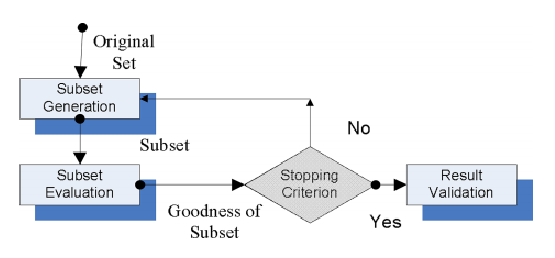
\includegraphics[width=0.5\textwidth]{featureSelection}
    \caption{Feature Selection}
    \label{fig:featureSelection}
\end{figure}
